\documentclass[letterpaper,10pt]{article}
\usepackage[utf8]{inputenc}
\usepackage{amsmath}
\usepackage{authblk}
\usepackage{graphicx}


\newcommand\blfootnote[1]{%
  \begingroup
  \renewcommand\thefootnote{}\footnote{#1}%
  \addtocounter{footnote}{-1}%
  \endgroup
}


\title{Sinking-point: Tracking floating-point precision with finitely many bits}
\author{Bill Zorn}
\author{Dan Grossman}
\author{Zach Tatlock}
\affil{University of Washington} 

\begin{document}

\maketitle

\blfootnote{This work was supported in part by Semiconductor Research Corporation (SRC).}

\begin{abstract}
 With its large dynamic range and ability to represent and compute with many real numbers in a small number of bits, floating-point arithmetic, as exemplified by the IEEE 754 floating-point standard, has become a critical tool for performing numerical computation. However, as with any finite approximation of the real numbers, floating-point introduces error into computations. This error is particularly insidious because it can be catastrophic in the worst case, it often occurs silently, and it is not compositional, making it difficult to analyze. To make floating-point error more tractable, we introduce sinking-point, a new floating-point arithmetic which dynamically tracks precision through a computation in a way that is compositional. Compared to typical floating-point arithmetics, sinking-point requires only a few extra bits and simple arithmetic operations, making it fast and amenable to implementation in hardware.
\end{abstract}


\section{Introduction}

Floating-point error is not compositional. That is to say, a sequence of operations, each of which produces little error on its own, might produce an overall error (when compared to the exact, real-valued result expected from the computation) of essentially unbounded size.

To illustrate, consider the computation $(3.14 + 10^{16}) - 10^{16}$. The order of evaluation is important here, because floating-point operations are not associative. When evaluated with real real numbers, where addition and subtraction are associative, we would expect the terms of $10^{16}$ to cancel and the result to be $3.14$. However, in a typical floating-point implementation which uses the IEEE 754 standard and a binary64 ``double precision'' representation, the computation returns a result of 4.

Despite this large overall error (the doubles closest to 3.14 and 4 don't even share the same exponent, and there are about $1.94 \times 10^{15}$ representable doubles between them), each individual addition and subtraction is computed as accurately as possible with the number of bits available. The IEEE 754 standard requires that basic arithmetic operations are correctly rounded to the nearest half-ulp (or Unit in the Last Place). The problem is that rounding off the low bits in the addition $3.14 + 10^{16}$, which seems inconsequential for a result of the same order of magnitude as $10^{16}$, suddenly becomes disasterous when subtracting another number of the same magnitude cancels most of the significant bits and leaves the result with a magnitude similar to the magnitude of the error.

Though the amount of error is not compositional, the amount of precision left in the computation is. The first addition rounds off the low bits of 3.14, but still leaves the full 53 bits of precision in the result; the subtraction cancels catastrophically and reduces the precision to only two bits. Floating-point implementations that follow the IEEE 754 standard will mask this loss of precision by filling out the low bits with zeros (as there is only one way to represent 4, and it has 53 bits of precision like every other non-subnormal number). This behavior makes some floating-point errors difficult to notice---without prior knowledge of the computation, 4 might seem like a perfectly reasonable and precise result. In contrast, sinking-point records the precision of each result. This way, it is immediately obvious when a result such as this 4 has been computed with low precision, and if that result is an intermediate used in further computation, future results will also be computed with low precision, rather than being silently and catastrophically wrong.

\section{Related Work}

Floating-point analysis is a rich area roughly between Programming Languages and Formal Methods. Tools such as Fluctuat \cite{fluctuat}, Rosa \cite{rosa}, and FPTaylor \cite{fptaylor} analyze floating-point programs statically. They can provide sound worst-case error bounds for small computations, but do not scale well to larger computations. Other tools such as Herbgrind \cite{herbgrind} and the work by Benz et al. \cite{benz2012dynamic} track floating-point error dynamically in computations, typically by keeping higher-precision ``shadow values.''

It is also worth mentioning the floating-point standards themselves, obviously the venerable IEEE 754 standard \cite{ieee754-2008}, as well as more recent work by John Gustafson on Posits \cite{beating754}, a similar standard designed to serve as a drop-in replacement for IEEE 754 floating-point.

Sinking-point is a combination of a floating-point standard and a dynamic analysis. Rather than keeping shadow values, which can be costly, it tracks precision by modifing the behavior of the arithmetic. As presented here, sinking-point is based on the IEEE 754 standard, but it can easily be adapted to work with any fixed or floating-point arithmetic, including Posits.

\section{Implementation}

In order to track precision in a compositional way, sinking-point needs to diverge from traditional IEEE 754 floating-point implementations in two ways. First, it needs to track the precision and exactness of each value, which can be done with at most $\log(p) + 1$ additional bits, where $p$ is the number of bits in the significand of the floating-point representation. Second, it needs to compute the output precision of each operation, based on the precision, exactness, and value of the inputs. This can be done with a handful of simple arithmetic operations, as shown in Table \ref{tab:rounding}.

\subsection{Floating-point rounding with $p$ and $n$}

To understand sinking-point's precision-management and rounding behavior, it is necessary to understand the rounding behavior of traditional IEEE 754 floating-point. We can express this behavior in terms of two quantities, $p$ and $n$, that express the precision of any floating-point number. $p$ is just the number of significant bits in the number's significand. For IEEE 754 floating-point numbers, this is a fixed number of bits for all non-subnormal numbers in some representation format - for binary64 ``double precision'' numbers, $p = 53$, including the implicit leading 1 bit.

$n$ is one less than the index of the least significant bit in a number. In other words, it is the first bit in an (inexact) number whose value is not known, or not recorded by the floating-point representation. For IEEE 754 formats, $n$ is always equal to the exponent of the number minus the number of bits in the representation's significand, or the smallest allowed exponent minus the number of bits in the representation's significand for subnormal numbers.

For example, consider the real number 1.25, which can be expressed as the binary fraction 0b1.01. This number has a 3-bit significand, so $p$ is 3. The exponent (in a typical IEEE 754 representation) is zero, so if the number is inexact, $n$ is $0 - 3 = -3$. This make sense; the first two bits after the binary place are known, but the third is not represented.

$n$ and $p$ convey different things about a given number's precision. $p$ gives the relative precision, compared to the exponent, that the number is known to; $n$ gives the absolute granularity of the number, or the distance from the next distinguishable number.

\subsection{Sinking-point rounding rules}

Rounding for some IEEE 754 format can be expressed as a maximum $p$ and minimum $n$: each result is rounded to at most $p$ bits of precision, and any bits below the minimum $n$ are cut off. No special cases are needed for subnormals; they are simply numbers that have some of their bits cut off due to the restriction on minimum $n$.

Rounding for sinking-point is slightly more complex. Instead of using a fixed maximum $p$ and minimum $n$ for every operation, $p_{max}$ and $n_{min}$ are computed according to the rules in Table \ref{tab:rounding}.

\begin{table} 
\begin{center}
\caption{Rounding rules for sinking-point} \label{tab:rounding}
\smallskip
\begin{tabular}{c|c|c}
 operation & $n$ & $p$ \\[5pt]
 \hline
 + & max($n_1$, $n_2$, $n_{min}$) & $p_{max}$ \\[5pt]
 - & max($n_1$, $n_2$, $n_{min}$) & $p_{max}$ \\[5pt]
 * & $n_{min}$ & min($p_1$, $p_2$, $p_{max}$) \\[5pt]
 / & $n_{min}$ & min($p_1$, $p_2$, $p_{max}$) \\[5pt]
 sqrt & $n_{min}$ & min($p_1$, $p_{max}$)
\end{tabular}

\smallskip

Subscripted variables $n_1$, $n_2$, $p_1$, and $p_2$ come from the corresponding inputs to the operation. $n_{min}$ and $p_{max}$ are taken from the overall IEEE 754-like format.
\end{center}
\end{table}

In addition to precision, sinking-point tracks the exactness of results. Exact numbers by definition do not have a finite precision: for an exact input, $p$ is treated as infinity and $n$ is treated as negative infinity. This way, operations with exact values that happen to have very compact representations will not cause unnecessary loss of precision.

Precision is a property of a rounded result. In general the precision of a result will never exceed the $p$ that was used by the rounding operation (unless the number was rounded up, and carried out of its most significant bit) and might be significantly less if bits are cut off due to limitations on $n$. Sinking-point must track the precision of results, avoiding the IEEE 754 behavior of silently padding unknown bits with zeros, out to maximum precision of the format.

Other than using different values of $n$ and $p$ and not padding imprecise results, the behavior of sinking point is indistinguishable from a typical implementation of the IEEE 754 format. $n_{min}$ and $p_{max}$ can be specified to limit results to finite precision in exactly the same way. Interestingly, the precision-limiting behavior of sinking-point can be bypassed by dropping the inexactness information and treating all values as exact. For a given $n_{min}$ and $p_{max}$, any operation with all exact inputs will produce the same result for both IEEE 754 and sinking-point arithmetics, though sinking-point may record different precision and exactness values.

\section{Experimental Results}

The correctness of sinking-point hinges on the compositionality of its precision tracking. For all operations, the precision of the output must not be more that the amount of precision that remains accurate when compared to the expected, real value.

We can test this emperically in the following way. For each input to an operation, we first generate a random value with some large reference precision. We then round each reference value to some small number of bits, our target precision, to produce a low-precision value. Performing the operation with both the high-precision reference inputs and the low-precision target inputs gives us a reference result and a target result. Using any IEEE 754-like format with at least as many bits of precision as our reference inputs will ensure both results are accurate, as we are only doing a single operation.

To determine the precision left in the target result, we compare it to the reference result, and find the largest number of bits such that if we rounded both results to that number of bits, they would be within one ulp of each other. For sinking point to be correct and demonstrate compositional precision tracking, it must never produce a result with more precision than this when given the target inputs.

Figure \ref{fig:add_scatter} shows a sweep over exponents in the range -14 to 15 and target precisions in the range 1 to 11, with 64 bits of reference precision and 10 random trials with each combination of exponent and target precision for each input. This sweep covers just over one million points, and is sufficient to cover every representable exponent and amount of precision for the IEEE 754 binary16 or ``half precision'' format. We plot the precision reported by sinking-point along the x axis, with the actual measured precision on the y axis. The intensity of each point represents the number of results that fall on that point. For correctness to hold, we expect to see points only at or above the line $y = x$, indicating that the actual precision is never less than what sinking-point reports.

\begin{figure}
\caption{Actual precision vs. reported precision for addition} \label{fig:add_scatter} \vspace{-10pt}
\begin{center}
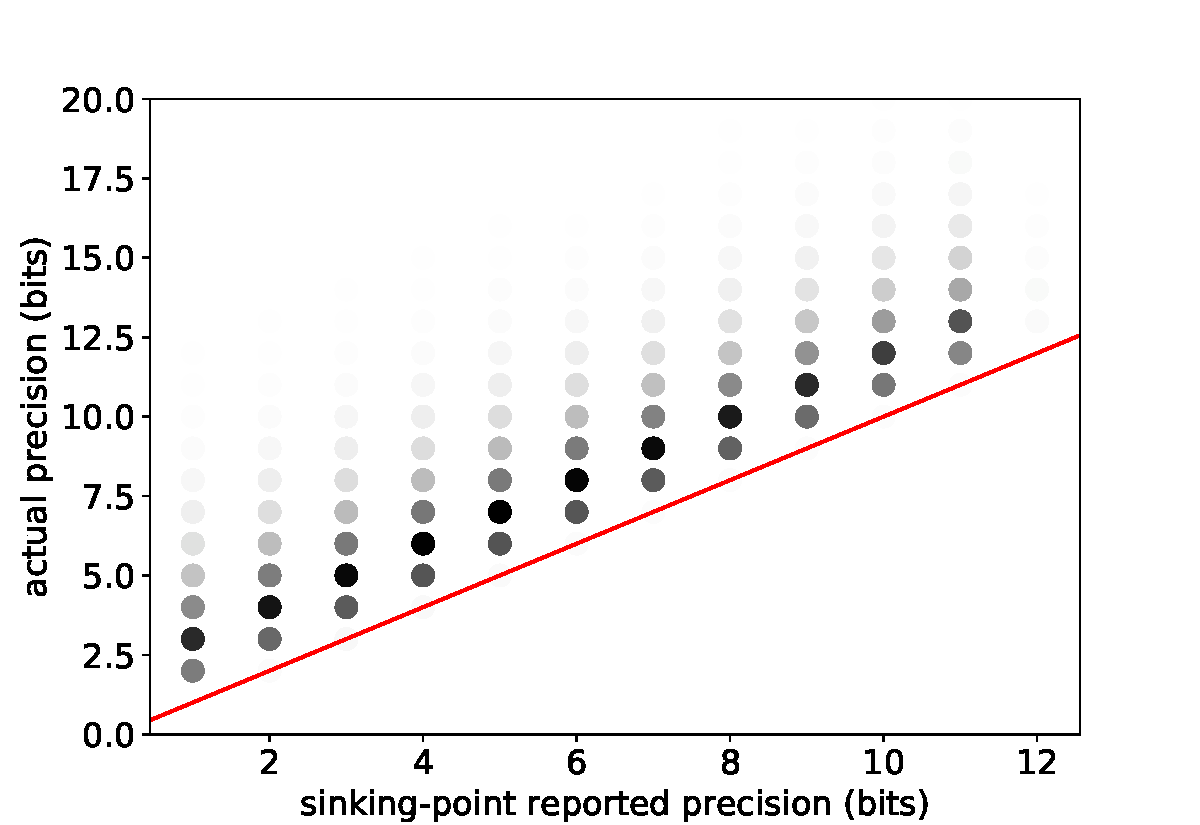
\includegraphics[width=0.75\textwidth]{add_scatter.pdf}
\end{center}
\end{figure}

\begin{figure}
\hspace{-.2\textwidth}
\begin{minipage}{1.2\textwidth}

 \begin{minipage}{0.6\textwidth}
  \begin{center} Figure 2a: CDF for addition \end{center} \vspace{-10pt}
  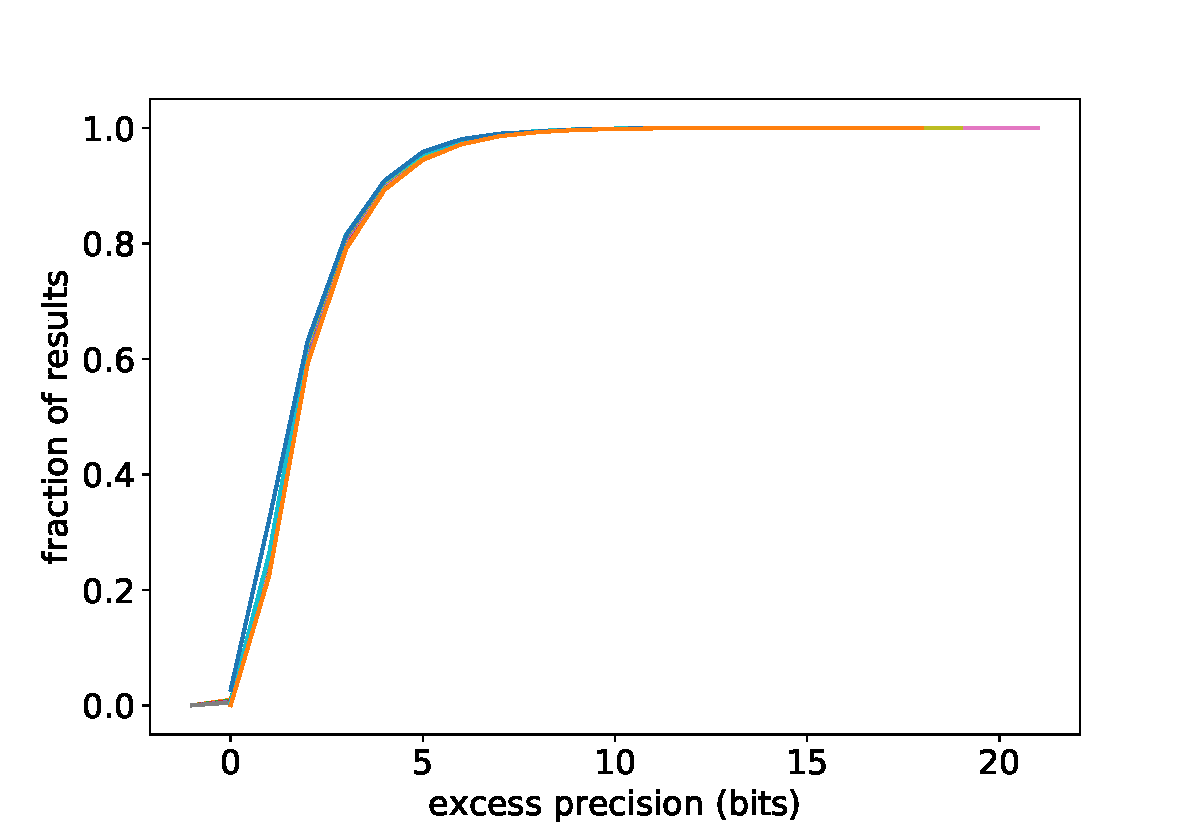
\includegraphics[width=1.0\textwidth]{add_cdf.pdf}
 \end{minipage}
 \begin{minipage}{0.6\textwidth}
  \begin{center} Figure 2b: CDF for subtraction \end{center} \vspace{-10pt}
  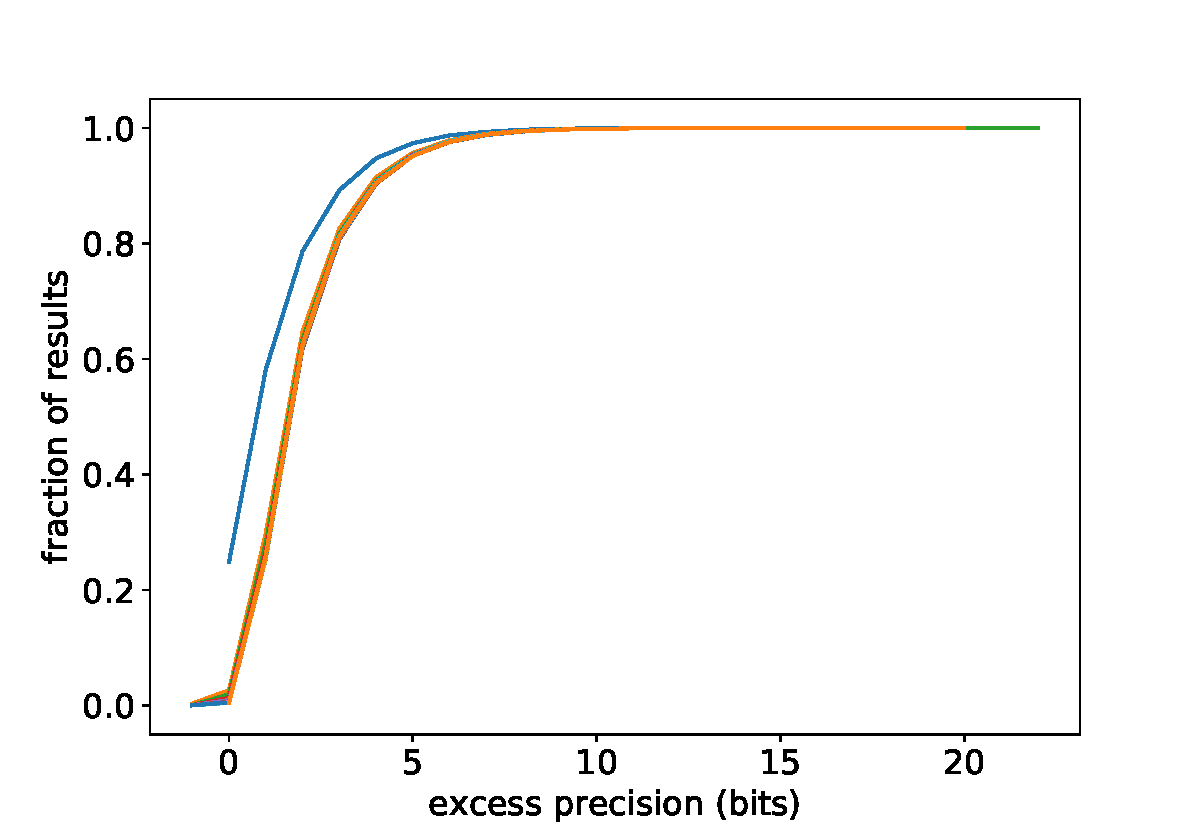
\includegraphics[width=1.0\textwidth]{sub_cdf.pdf}
 \end{minipage}
 
 \bigskip
 
 \begin{minipage}{0.6\textwidth}
  \begin{center} Figure 2c: CDF for multiplication \end{center} \vspace{-10pt}
  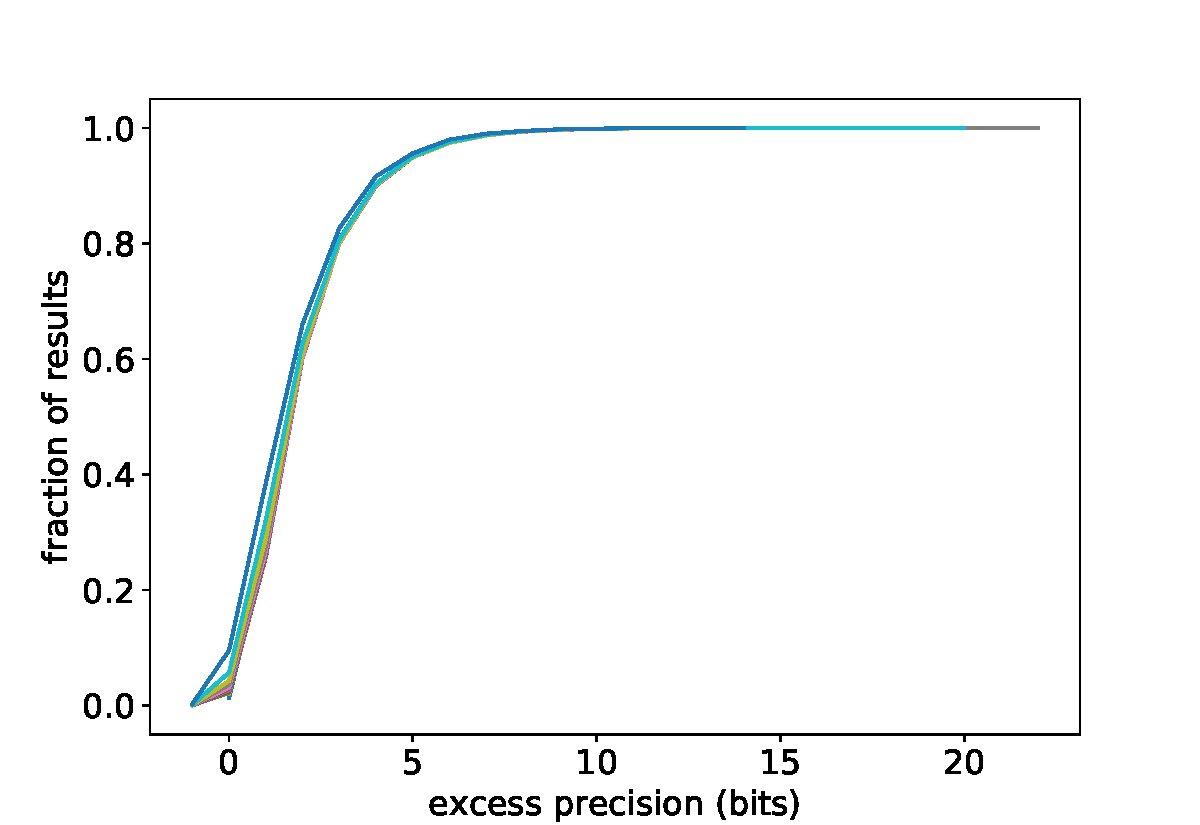
\includegraphics[width=1.0\textwidth]{mul_cdf.pdf}
 \end{minipage}
 \begin{minipage}{0.6\textwidth}
  \begin{center} Figure 2d: CDF for division \end{center} \vspace{-10pt}
  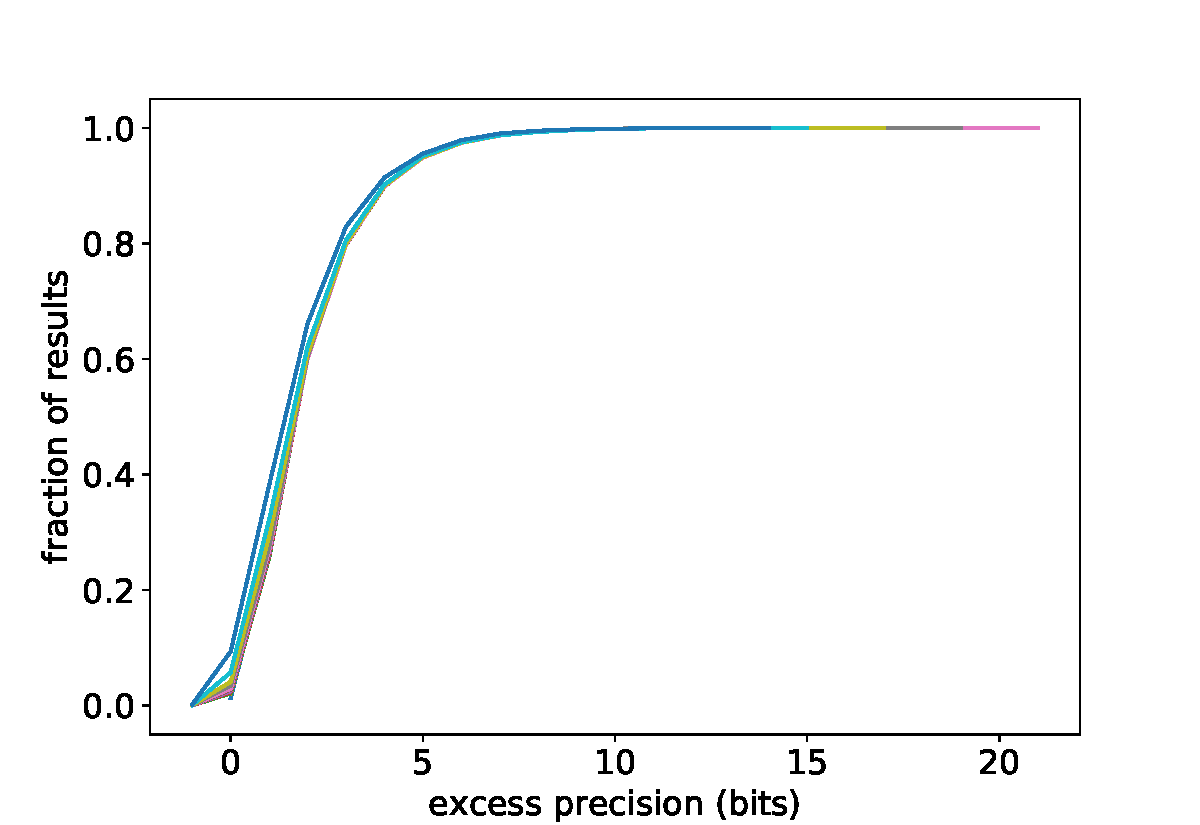
\includegraphics[width=1.0\textwidth]{div_cdf.pdf}
 \end{minipage}
 
 \smallskip
 
 \begin{center}
 \begin{minipage}{0.6\textwidth}
  \begin{center} Figure 2e: CDF for square root \end{center} \vspace{-10pt}
  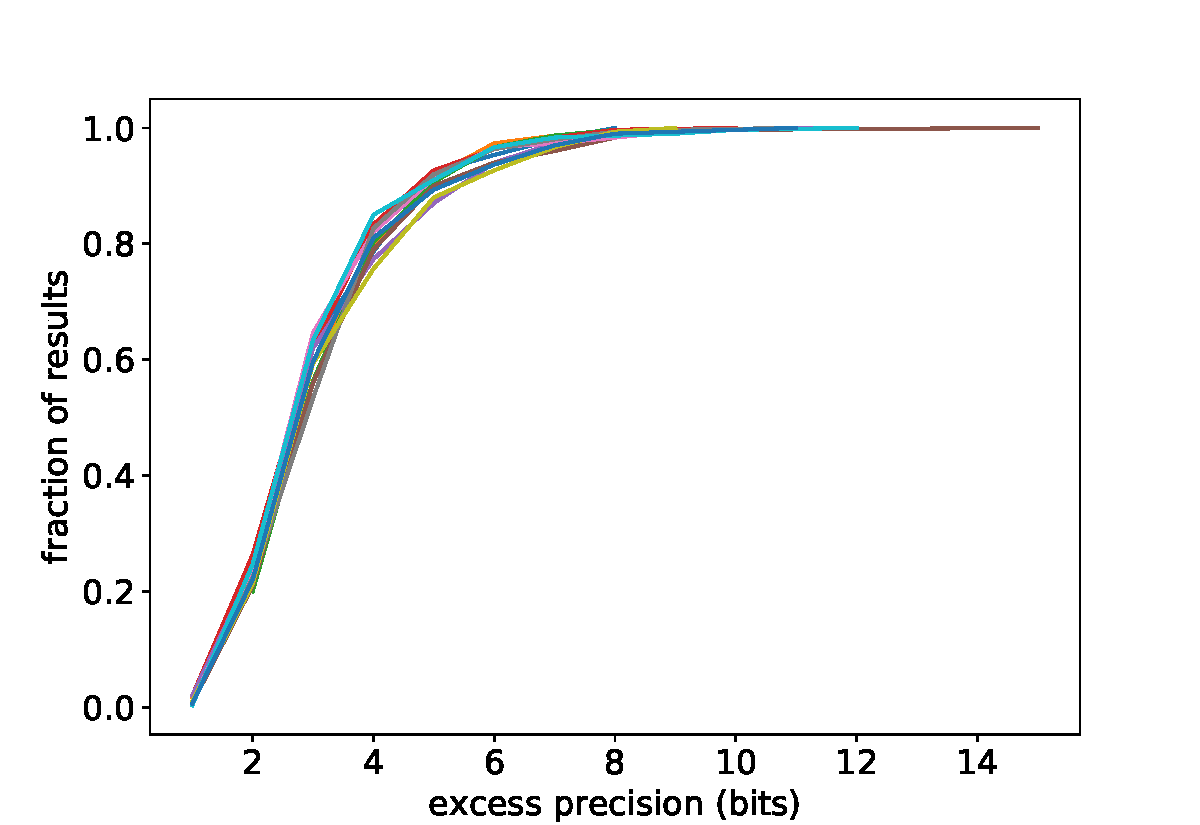
\includegraphics[width=1.0\textwidth]{sqrt_cdf.pdf}
 \end{minipage}
 \end{center}

\end{minipage}
\end{figure}

We can make this data more intelligible by plotting a CDF of the excess precision, or the difference between the actual precision and the reported precision, for each value of the reported precision. We expect each line to quickly converge to 1, which would indicate that we are wasting as few bits as possible by reporting less precision than is actually observed. To show correctness, we want each line to have no mass below 0. CDFs for each operation are shown in Figures 2a-2e, with the same sweep parameters used in Figure \ref{fig:add_scatter}.


Several important points should be made about the graphs. First, in some cases sinking point reports one more bit of precision than is observed, leading to some probability mass below 0. This is due to results rounding up and carrying out of the most significant bit, which produces a result with an extra bit of precision.

Second, based on the CDFs, it would seem that sinking-point is throwing away a lot of precision, 4 or 5 bits in up to 20\% of operations. These tests represent something of a worst case scenario for sinking point: the inputs are always inexact, and one is usually much more precise than the other. By random chance, we would expect the bits in the rounded results to agree half of the time, so the CDF should never converge faster than 50\% per bit. Since one of the inputs will usually have some accurate bits, we would actually expect it to converge more slowly.

\section{Conclusion}

We have presented sinking-point, a floating-point like arithmetic that tracks precision in a compositional way. Like traditional floating-point arithmetics, sinking-point uses a finite representation with a small number of bits, and its arithmetic operations are not significantly more expensive to compute or implement in hardware. By clearing the exactness metadata for values, it is trivial for sinking-point to reproduce the behavior of the IEEE 754 standard, or any other floating-point arithmetic that it is based on.

Like floating-point, sinking-point is not formally sound. There exist computations and inputs where sinking-point will still produce the wrong answer with relatively high precision, or where it will report low precision even though the result could have been computed accurately. However, the guarantees it provides are much stronger than floating-point.

Traditionally, floating point formats have been designed to pack as many representable numbers into as few bits as possible. Sinking-point is a step in a different direction. Modern computers have no shortage of bits; using a few of them to track precision could be invaluable to safety-critical programs, or any applications where numerical accuracy is important.


\bibliographystyle{ieeetr}
\bibliography{ref}

\end{document}
